\subsection{Red-Black Trees}

I \emph{Red-Black Trees} sono ABR i cui nodi hanno un campo \emph{colore} $x.color$, che può essere:
\begin{itemize}[noitemsep]
    \item $\const{red}$ per il rosso;
    \item $\const{black}$ per il nero.
\end{itemize}

\paragraph{Accorgimento} $\const{nil}$ sarà in realtà un nodo,
$T.nil$, con $T.nil.color = \const{black}$.

\paragraph{Caratteristiche} \emph{RB-tree} è in realtà un ABR tale che:
\begin{enumerate}[label=($\arabic*$)]
    \item Ogni nodo $x$ ha $x.color \in \{\const{red},\const{black}\}$; \label{rbtree:1}
    \item La radice $root$ è $\const{black}$; \label{rbtree:2}
    \item Le foglie ($T.nil$) sono $\const{black}$; \label{rbtree:3}
    \item Se $x$ è $\const{red}$, i figli sono $\const{black}$; \label{rbtree:4}
    \item Per ogni nodo $x$, ogni cammino da $x$ a una qualsiasi delle foglie
    ha lo stesso numero di nodi $\const{black}$ (calcolato con $bh(x)$). \label{rbtree:5}
\end{enumerate} 

\begin{figure}[hbt]
    \centering
    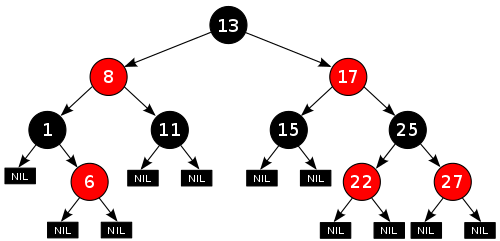
\includegraphics[width=\textwidth]{img/rb-tree-ex.png}
    \caption{Esempio di un RB-tree.}
\end{figure}
\pagebreak

È possibile notare che: 
\begin{itemize}
    \item In caso non ci fossero nodi rossi, avremo un albero
    perfettamente bilanciato;
    \item In ogni cammino, il \verb|#| di nodi $\const{black}$ è almeno la
    metà del \verb|#| dei nodi $\const{red}$
\end{itemize}

\paragraph{Osservazione} Se $T$ è un \emph{RB-tree} con $n$ nodi interni ($\neq \const{nil}$)
e $h$ altezza, allora vale
$$h \leq 2 \log (n + 1)$$

\subparagraph{Dimostrazione} Consideriamo 
$$n_x \geq 2^{bh(x)} - 1$$
La dimostrazione è per induzione su $h_x$ (altezza del sotto-albero radicato in $x$).

\begin{description}
    \item[$(h_x = 1)$] Allora ho solo 
    $T.nil \Rightarrow n_x = 0 = 2^0 - 1 \qquad (2^0 \text{ con } 0 = bh(x))$
    \item[$(h_x > 1)$] Consideriamo $x$ radice. $x$ ha due figli, $x_1$ e $x_2$.\par
    Sicuramente vale $h_1,h_2 < h$. Per ipotesi induttiva, valgono:
    $$n_{x_1} \geq 2^{bh(x_1)} - 1$$
    $$n_{x_2} \geq 2^{bh(x_2)} - 1$$
    \begin{align*}
        n_x & = n_{x_1} + n_{x_2} + 1 \\
        & \geq 2^{bh(x_1)} + 2^{bh(x_2)} - 1 \\
        & \geq 2 \cdot 2^{bh(x)-1} - 1 = 2^{bh(x)} - 1 \\
        & \qquad (\text{valgono } bh(x_1) \geq bh(x)-1, \ bh(x_2) \geq bh(x)-1) \\
        \text{Comples}&\text{sivamente}\\
        n & = n_{root} \geq 2^{bh(root)} - 1
    \end{align*}
    Essendo $bh(root) \geq \frac{h}{2}$, posso ottenere
    \begin{align*}
        n_{root} & \geq 2^{bh(root)} - 1 \\
        & 2^{\frac{h}{2}} - 1 \\
        \Rightarrow \ & 2^{\frac{h}{2}} \leq n + 1 \\
        & \frac{h}{2} \leq \log_2(n+1) \Rightarrow h \leq 2 \log_2(n+1) 
    \end{align*}
\end{description}

\subsubsection{Complessità Algoritmi RB-Trees}
\texttt{Search, Succ, Min, Pred, Max} hanno complessità $O(h) = O(\log n)$

\subsubsection{RB-Insert e RB-Delete}
A differenza di quelle citate precedentemente, che risultano semplici
sia come complessità asintotica che come implementazione, bisogna porre 
particolare attenzione a queste due procedure: \texttt{RB-Insert} e \texttt{RB-Delete}.

Per ovviare a ciò, posso utilizzare le \emph{rotazioni}. Consideriamo il seguente albero,
in cui $x$ e $y$ sono nodi normali, mentre $\alpha, \ \beta$ e $\gamma$ sono sotto-alberi
(il colore dei nodi non ha importanza ai fini della procedura che andremo a 
vedere)\footnote{Di conseguenza, applicandola a un \emph{RB-tree}, gli assiomi di validità potrebbero venire violati.}:
\begin{center}
	\begin{tikzpicture}[tree]
	\Tree
	[.$x$     
		[.$\alpha$ ]
		[.$y$ 
            [.$\beta$ ]
			[.$\gamma$ ]
        ]
	]
	\end{tikzpicture}
\end{center}
Applichiamo \texttt{Left(T,x)}, ottenendo:
\begin{center}
	\begin{tikzpicture}[tree]
	\Tree
	[.$y$
        [.$x$
            [.$\alpha$ ]
            [.$\beta$ ]
		]
		[.$\gamma$ ]
	]
	\end{tikzpicture}
\end{center}

\paragraph{Osservazione} La \emph{visita simmetrica} è identica per i due alberi:
$$\alpha \rightarrow x \rightarrow \beta \rightarrow y \rightarrow \gamma$$

\paragraph{RB-Insert(T, z)} Voglio inserire $z$ nell'albero $T$.
L'idea è quella di porre $z.color = \const{red}$ poichè meno insidioso\footnote{Andando a modificare il numero di nodi neri, cambia l'altezza nera, e la cosa è difficile da sistemare.}.
\begin{itemize}
    \item Se violo \ref{rbtree:2} $\Rightarrow z.color = \const{black}$;
    \item Se violo \ref{rbtree:4}:
    \begin{itemize}
        \item Risolvo localmente;
        \item Sposto verso l'alto il problema.
    \end{itemize}
\end{itemize}

Abbiamo due \emph{macrocasi}. $z.p$ è figlio sinistro, oppure destro. Noi analizzeremo solo il primo: \textbf{z.p figlio sinistro}\footnote{I nodi non cerchiati sono $\const{red}$, %
	quelli cerchiati sono $\const{black}$, quelli tratteggiati e puntinati possono essere sia $\const{red}$ che $\const{black}$.}.
\begin{center}
	\begin{tikzpicture}[tree]
	\Tree
	[.$z.p.p$
        [.\node[red]{$z.p$};
            [.\node[red]{$z$}; ]
		]
		[.\node[unknown]{$y$}; ]
    ]
	\end{tikzpicture}
\end{center}

Abbiamo due possibilità per $y$:
\begin{enumerate}
    \item $y.color = \const{red}$. Inverto il colore di $z.p.p$ con quello dei figli, ottenendo:
    \begin{center}
        \begin{tikzpicture}[tree]
        \Tree
        [.\node[red]{$z.p.p$};
            [.$z.p$
                [.\node[red]{$z$}; ]
            ]
            [.$y$ ]
        ]
        \end{tikzpicture}
    \end{center}
    In questo modo, risolviamo localmente e rimandiamo il problema in alto.
    \item $y.color = \const{black}$. Possiamo distinguere due sottocasi:
    \begin{enumerate}[label=($2.\arabic*$)]
        \item $z$ figlio destro. \label{rbinsert:2.1}
        \begin{center}
            \begin{tikzpicture}[tree]
            \Tree
            [.$z.p.p$
                [.\node[red]{$z.p$};
                    \edge[blank]; \node[blank]{};
                    [.\node[red]{$z$}; ]
                ]
                [.$y$ ]
            ]
            \end{tikzpicture}
        \end{center}
        Applico \texttt{Left(T,z.p)}, ottenendo:
        \begin{center}
            \begin{tikzpicture}[tree]
            \Tree
            [.$z.p.p$
                [.\node[red]{$z$};
                    [.\node[red]{$z.p$}; ]
                    \edge[blank]; \node[blank]{};
                ]
                [.$y$ ]
            ]
            \end{tikzpicture}
        \end{center}
    	Mi riconduco al caso \ref{rbinsert:2.2}. 

        \item $z$ figlio sinistro. \label{rbinsert:2.2}
        \begin{center}
            \begin{tikzpicture}[tree]
            \Tree
            [.$z.p.p$
                [.\node[red]{$z.p$};
                    [.\node[red]{$z$}; ]
                    \edge[blank]; \node[blank]{};
                ]
                [.$y$ ]
            ]
            \end{tikzpicture}
        \end{center}
        Scambio i colori di $z.p.p$ con $z.p$, ottenendo:
        \begin{center}
            \begin{tikzpicture}[tree]
            \Tree
            [.\node[red]{$z.p.p$};
                [.$z.p$
                    [.\node[red]{$z$}; ]
                    \edge[blank]; \node[blank]{};
                ]
                [.$y$ ]
            ]
            \end{tikzpicture}
        \end{center}
        Applico \texttt{Right(T,z.p.p)}\footnote{Analoga di \texttt{Left}.}, ottenendo:
        \begin{center}
            \begin{tikzpicture}[tree]
            \Tree
            [.$z.p$
                [.\node[red]{$z$}; ]
                [.\node[red]{$z.p.p$}; 
                    \edge[blank]; \node[blank]{};
                    [.$y$ ]
                ]
            ]
            \end{tikzpicture}
        \end{center}
    \end{enumerate}
\end{enumerate}

\begin{codebox}
\Procname{\proc{RB-Insert}$(T,z)$}
\li $\proc{Insert}(T,z)$
\li $\attrib{z}{color} \gets \const{red}$
\li $\proc{RB-Insert-Fixup}(T,z)$
\end{codebox}
\begin{codebox}
\Procname{\proc{RB-Insert-Fixup}$(T,z)$}
\li \While $\attrib{\attrib{z}{p}}{color} = \const{red}$
\li \Do
        \If $\attrib{z}{p} = \attrib{\attrib{\attrib{z}{p}}{p}}{left}$
        \Comment Macrocaso $z.p$ figlio sinistro
\li     \Then
            $y \gets \attrib{\attrib{\attrib{z}{p}}{p}}{right}$
\li         \If $\attrib{y}{color} = \const{red}$ \Comment Caso 1
\li         \Then
                $\attrib{\attrib{\attrib{z}{p}}{p}}{color} \gets \const{red}$
\li             $\attrib{\attrib{z}{p}}{color} \gets \const{black}$
\li             $\attrib{y}{color} \gets \const{black}$
\li             $z \gets \attrib{\attrib{z}{p}}{p}$
\li         \Else \Comment Caso 2
\li             \If $z = \attrib{\attrib{z}{p}}{right}$ \Comment Caso \ref{rbinsert:2.1}
\li             \Then
                    $\proc{Left}(T,\attrib{z}{p})$
\li                 $z \gets \attrib{z}{left}$
                \End
\zi             \Comment Caso \ref{rbinsert:2.2}
\li             $\attrib{\attrib{z}{p}}{color} \gets \const{black}$
\li             $\attrib{\attrib{\attrib{z}{p}}{p}}{color} \gets \const{red}$
\li             $\proc{Right}(T,\attrib{\attrib{z}{p}}{p})$
            \End
\li     \Else $\dots$ \Comment Macrocaso $z.p$ figlio destro
        \End
    \End
\li $\attrib{\attrib{T}{root}}{color} \gets \const{black}$
\end{codebox}

\subparagraph{Complessità} $O(\log n) + \text{max } 2$ rotazioni

\paragraph{RB-Delete(T, z)} Distinguiamo 2 casi:
\begin{enumerate}[label=($\arabic*$)]
	\item $z$ ha un figlio;
	\item $z$ ha due figli.
\end{enumerate}
Ci comportiamo allo stesso modo della \texttt{Delete(T,z)} per un ABR, facendo però un'ulteriore accorgimento:
\begin{itemize}
	\item se $z.color = \const{red}$ non ho problemi
	\item se $z.color = \const{black}$ violo \ref{rbtree:5}:
	\begin{itemize}
		\item Risolvo localmente;
		\item Sposto verso l'alto il problema.
	\end{itemize}
\end{itemize}
Dunque, in seguito alla \texttt{Delete(T,z)}, il nodo $x$ che ha preso il posto di $z$ ne ''assorbirà'' il colore diventando doppiamente $\const{black}$. \par
Abbiamo due \emph{macrocasi}. $x$ è figlio sinistro, oppure destro. Noi analizzeremo solo il primo: \textbf{x figlio sinistro}.
\begin{center}
	\begin{tikzpicture}[tree]
	\Tree
	[.\node[unknown]{$x.p$};
		[.\node[double circle]{$x$}; ]
		[.\node[unknown]{$w$}; ]
	]
	\end{tikzpicture}
\end{center}
Abbiamo due possibilità per $w$:
\begin{enumerate}
	\item $w.color = \const{red}$ \label{rbdelete:1}
	\begin{center}
		\begin{tikzpicture}[tree]
		\Tree
		[.$x.p$
			[.\node[double circle]{$x$}; ]
			[.\node[red]{$w$};
				[.\scriptsize $w.left$ ]
				[.\scriptsize $w.right$ ]
			]
		]
		\end{tikzpicture}
	\end{center}
	Scambio i colori di $w$ con $x.p$, ottenendo:
	\begin{center}
		\begin{tikzpicture}[tree]
		\Tree
		[.\node[red]{$x.p$};
			[.\node[double circle]{$x$}; ]
			[.$w$
				[.\scriptsize $w.left$ ]
				[.\scriptsize $w.right$ ]
			]
		]
		\end{tikzpicture}
	\end{center}
	Applico \texttt{Left(T,x.p)}, ottenendo:
	\begin{center}
		\begin{tikzpicture}[tree]
		\Tree
		[.$w$
			[.\node[red]{$x.p$};
				[.\node[double circle]{$x$}; ]
				[.\scriptsize $w.left$ ]
			]
			[.\scriptsize $w.right$ ]
		]
		\end{tikzpicture}
	\end{center}
	Mi riconduco al caso \ref{rbdelete:2}

	\item $w.color = \const{black}$ \label{rbdelete:2}
	\begin{center}
		\begin{tikzpicture}[tree]
		\Tree
		[.\node[red]{$x.p$};
			[.\node[double circle]{$x$}; ]
			[.$w$
				[.\node[red]{\scriptsize $w.left$}; ]
				[.\node[red]{\scriptsize $w.right$}; ]
			]
		]
		\end{tikzpicture}
	\end{center}
	Possiamo distinguere tre sottocasi:
	\begin{enumerate}[label=($2.\arabic*$)]
		\item $w.left.color = \const{black}$ e $w.right.color = \const{black}$ \label{rbdelete:2.1}
		\begin{center}
			\begin{tikzpicture}[tree]
			\Tree
			[.\node[unknown]{$x.p$};
				[.\node[double circle]{$x$}; ]
				[.$w$
					[.\scriptsize $w.left$ ]
					[.\scriptsize $w.right$ ]
				]
			]
			\end{tikzpicture}
		\end{center}
		$x$ cede un suo \const{black} a $x.p$ e $w$ diventa per forza $\const{red}$, ottenendo:
		\begin{center}
			\begin{tikzpicture}[tree]
			\Tree
			[.\node[double circle={4pt}{unknown}]{$x.p$};
				[.$x$ ]
				[.\node[red]{$w$};
					[.\scriptsize $w.left$ ]
					[.\scriptsize $w.right$ ]
				]
			]
			\end{tikzpicture}
		\end{center}
		In questo modo, risolviamo localmente e rimandiamo il problema in alto.
		
		\item $w.right.color = \const{black}$ \label{rbdelete:2.2}
		\begin{center}
			\begin{tikzpicture}[tree]
			\Tree
			[.\node[unknown]{$x.p$};
				[.\node[double circle]{$x$}; ]
				[.$w$
					[.\node[red]{\scriptsize $w.left$}; ]
					[.\scriptsize $w.right$ ]
				]
			]
			\end{tikzpicture}
		\end{center}
		Scambio i colori di $w$ con $w.left$, ottenendo:
		\begin{center}
			\begin{tikzpicture}[tree]
			\Tree
			[.\node[unknown]{$x.p$};
				[.\node[double circle]{$x$}; ]
				[.\node[red]{$w$};
					[.\scriptsize $w.left$ ]
					[.\scriptsize $w.right$ ]
				]
			]
			\end{tikzpicture}
		\end{center}
		Applico \texttt{Right(T,w)}, ottenendo:
		\begin{center}
			\begin{tikzpicture}[tree]
			\Tree
			[.\node[unknown]{$x.p$};
				[.\node[double circle]{$x$}; ]
				[.\scriptsize $w.left$
					\edge[blank]; \node[blank]{};
					[.\node[red]{$w$};
						\edge[blank]; \node[blank]{};
						[.\scriptsize $w.right$ ]
					]
				]
			]
			\end{tikzpicture}
		\end{center}
		Mi riconduco al caso \ref{rbdelete:2.3}
		
		\item $w.right.color = \const{red}$ \label{rbdelete:2.3}
		\begin{center}
			\begin{tikzpicture}[tree]
			\Tree
			[.\node[unknown]{$x.p$};
				[.\node[double circle]{$x$}; ]
				[.$w$
					[.\node[unknown2]{\scriptsize $w.left$}; ]
					[.\node[red]{\scriptsize $w.right$}; ]
				]
			]
			\end{tikzpicture}
		\end{center}
		Scambio i colori di $x.p$ con $w$ e $w.right$ diventa $\const{black}$, ottenendo:
		\begin{center}
			\begin{tikzpicture}[tree]
			\Tree
			[.$x.p$
				[.\node[double circle]{$x$}; ]
				[.\node[unknown]{$w$};
					[.\node[unknown2]{\scriptsize $w.left$}; ]
					[.\scriptsize $w.right$ ]
				]
			]
			\end{tikzpicture}
		\end{center}
	Applico \texttt{Left(T,x.p)}, ottenendo:
	\begin{center}
		\begin{tikzpicture}[tree]
		\Tree
		[.\node[unknown]{$w$};
			[.$x.p$
				[.\node[double circle]{$x$}; ]
				[.\node[unknown2]{\scriptsize $w.left$}; ]
			]
			[.\scriptsize $w.right$ ]
		]
		\end{tikzpicture}
	\end{center}
	Ho risolto.
	\end{enumerate}
\end{enumerate}

\subparagraph{Complessità} $O(\log n) + \text{max } 3$ rotazioni
